\section{Eksperimenti 1. faze}

\subsection{Določevanje zakasnitve fiziološkega odziva}

We explored the problem of the lag in physiological response as well. Based on Figure \ref{fig:zakasnitev}, we found out that between the change in speed of the treadmill and change of the selected physiological parameter there is a delay. This is perfectly acceptable due to the nature of physiological processes. We found out that offset for heart rate is amounted to \SI{15}{\s} and for energy expenditure to \SI{55}{\s}. Offset was included in models with the \textit{lag} abbreviation.

\begin{figure}[htb]
\centering
\begin{subfigure}[t]{0.45\columnwidth}
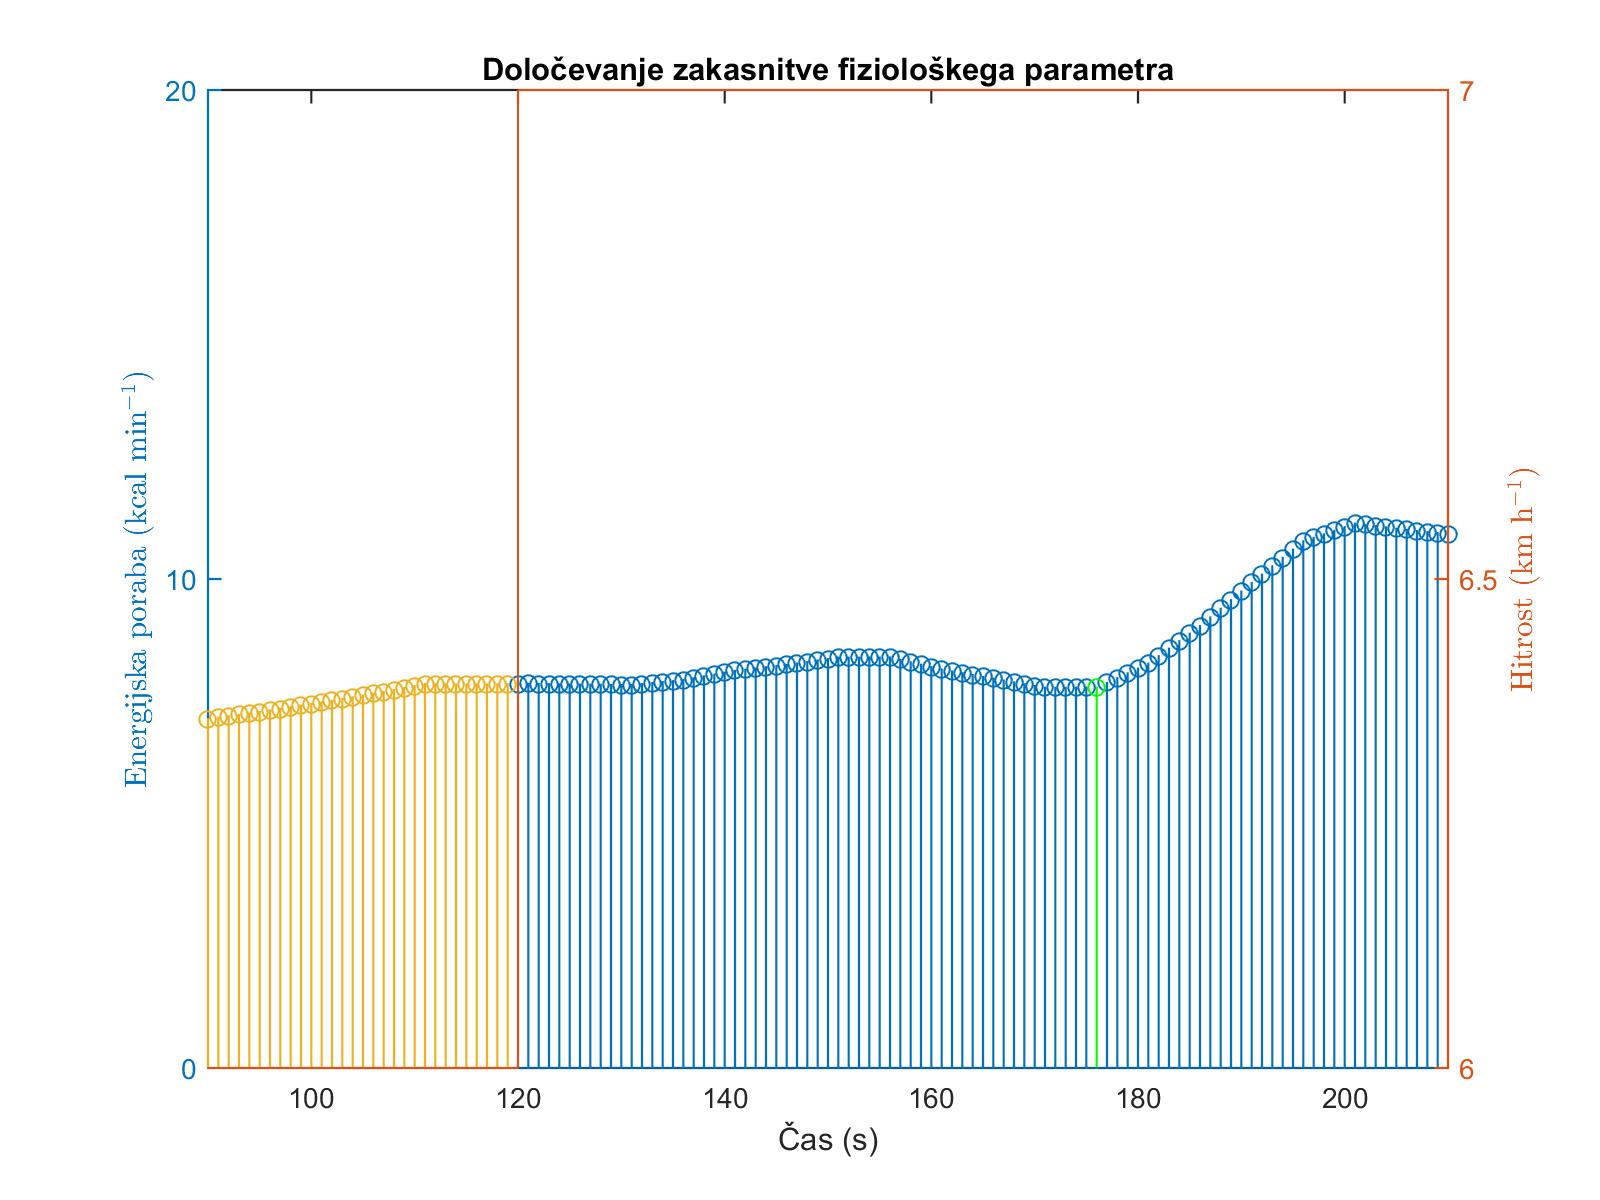
\includegraphics[width=\columnwidth]{./Slike/lag-estimation-train-eem.png}
\caption{Zakasnitev za energijsko porabo.}
\label{fig:lag-estimation-train-eem}
\end{subfigure}
~
\begin{subfigure}[t]{0.45\columnwidth}
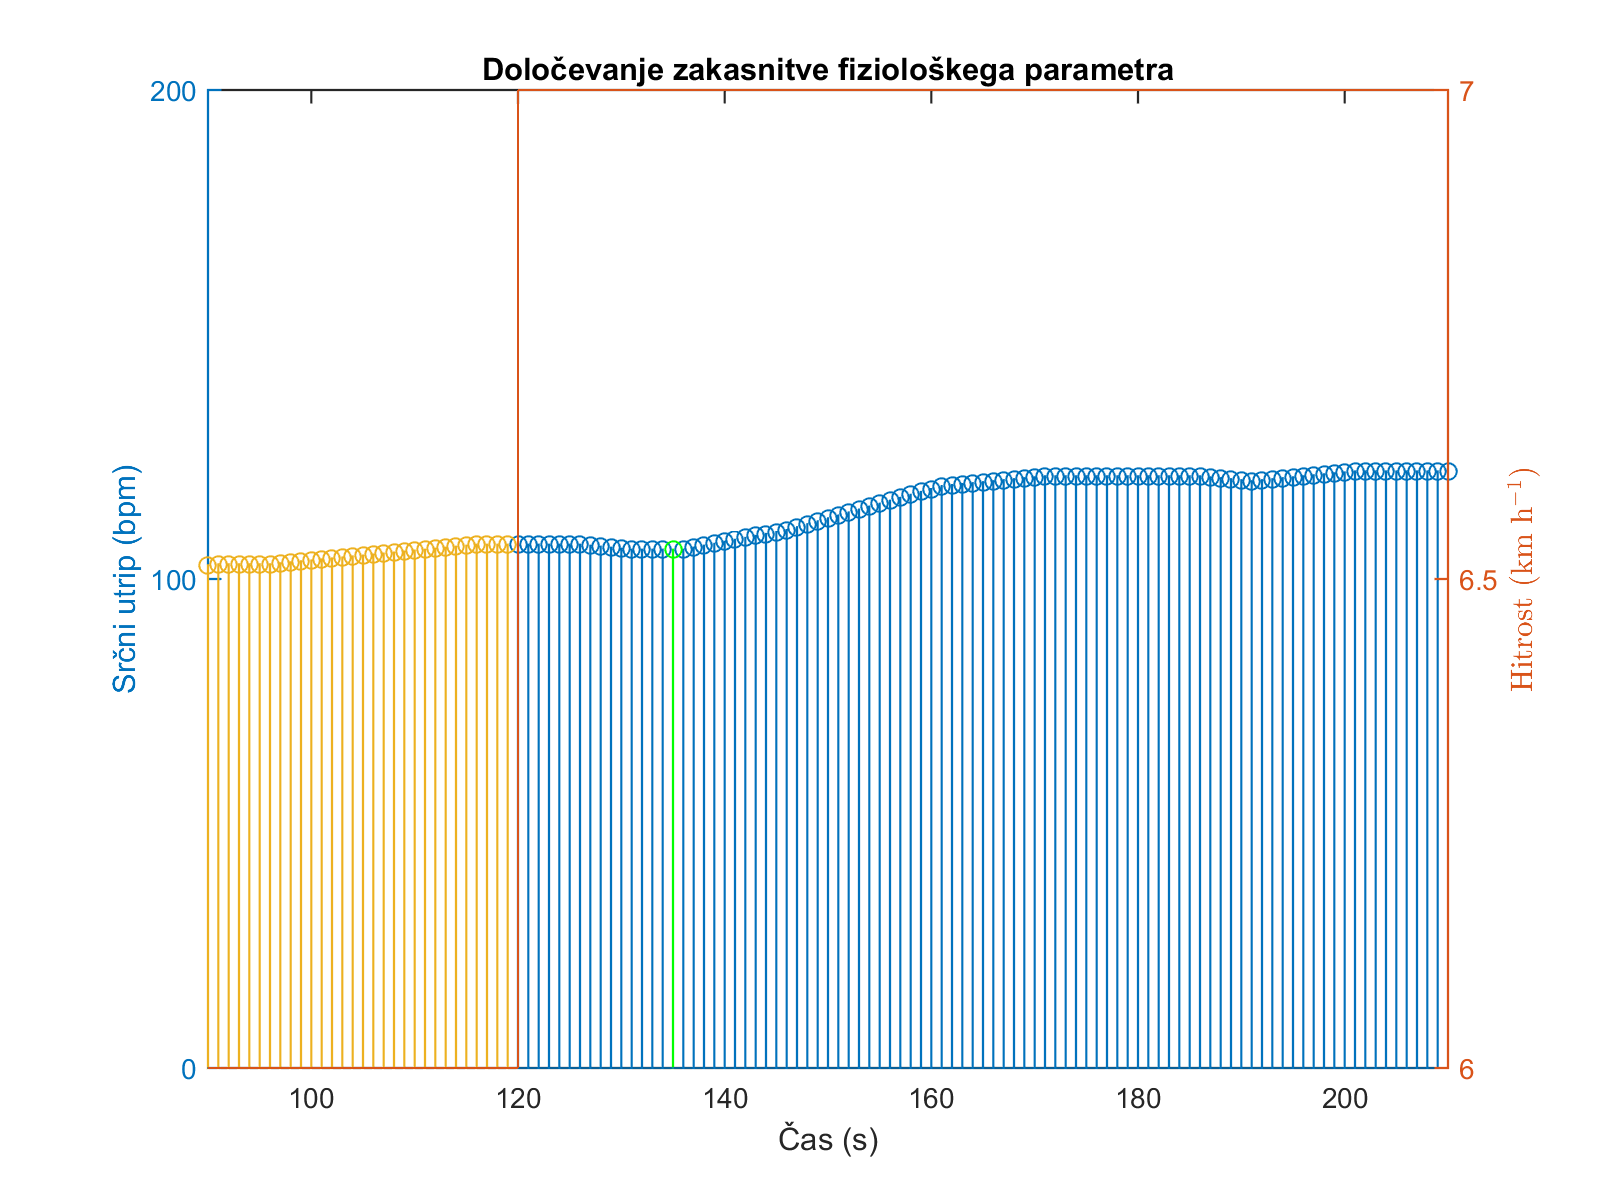
\includegraphics[width=\columnwidth]{./Slike/lag-estimation-train-hr.png}
\caption{Zakasnitev za srčni utrip.}
\label{fig:lag-estimation-train-hr}
\end{subfigure}
\caption{}
\label{fig:lag-estimation-stage1}
\end{figure}


\subsubsection{Normalizacija HAFA deskriptorjev}
% Zakaj naj bi bila ta rešitev dobra
% teorija tovrstne kalibracije
% Kako s to kalibracijo nismo popravili stvari
% In da smo ugotovili da obstaja še prostorski tok, ki bi nam rešil težave
!!!!!!!!!!!!!!!!!!!!!!!!!!!!!!!

V praksi se pokaže, da normiran HAFA histogram ne... -> To paše pod eksperimente.

!!!!!!!!!!!!!!!!!!!!!!!!!!!!!!!!!!!!!!!!!


\subsection{Treadmill experiment}
The first set of experiments was performed in physiological laboratory, with subject running on a treadmill in the presence of the operator---a doctor, who determined the intensity and duration of workload. Heart rate and energy expenditure were measured for an athlete (age: 26 years, height: \SI{177}{\cm}, weight: \SI{79.1}{\kg}, $VO_2max$: \SI{3705}{\ml\per\min}). Energy expenditure was measured using indirect calorimetry with Cosmed CPET Metabolic Cart. System allows breath-by-breath measurement \cite{beaver1973line}. We used Hans Rudolph face mask with prescribed minimal VD (dead space).

\subsubsection{Data acquisition}
We filmed the treadmill from the two different angles: the side-view and the back-view. The slope of the treadmill was from \SI{1.5}{\%} to \SI{2}{\%}. We filmed in $480 \times 640$ resolution with a \SI{30}{fps} speed. An example of a recording is shown in Figure \ref{fig:moving-components}(\subref{fig:original-frame}).

\subsubsection{Procedure}
We have made two series of tests with 20 minutes between them. Physiological parameters were sampled every \SI{5}{\s}. In the first series we made 8 tests, where every test lasted for 2 minutes. The treadmill's speed was increased by \SI{1}{\km\per\hour} every test. First test had a speed of \SI{6}{\km\per\hour} and the last a speed of \SI{13}{\km\per\hour}. In the second series we made 3 tests. Every test lasted for 5 minutes. Treadmill's speeds were \SI{7}{\km\per\hour}, \SI{10}{\km\per\hour} and \SI{13}{\km\per\hour}. The first set was used for the acquisition of samples for learning, and the other for testing.

\subsubsection{Processing}
We then calculated the optical flow \cite{farneback2003two} with the help of tracking algorithm described in \ref{sec:tracking}. For optical flow we used the following parameters: pyramid scale \num{0.5}, number of pyramid layers \num{3}, averaging window size \num{15}, number of iterations at each pyramid level \num{3}, size of the pixel neighborhood \num{5} and standard deviation of the Gaussian \num{1.2}. An example of the obtained optical flow is shown in Figure \ref{fig:optical-flow}.

\begin{figure}[!htb]
	\centering
	%\includegraphics[width=0.75\linewidth, frame]{./slike/colored-opticalFlow-frame-150.png}
    \caption{The optical flow for $150^{\mathrm{th}}$ frame of the first test from the first series of shots with color coding legend in the bottom left corner. We are using a standard color coding based on \cite{baker2011database}. The maximum amplitude of the optical flow in this figure is \SI{17}{px}.}
    \label{fig:optical-flow}
\end{figure}

HOOF features were calculated according to the method described in \cite{chaudhry2009histograms}.

The models have been generated with support vector regression \mbox{$\epsilon$-SVR} in LIBSVM library, which is more specifically described in \cite{CC01a}. We used RBF kernel that takes the form \eqref{eq:rbf-kernel}. Kernel and regression parameters were optimized with grid search approach described in \cite{hsu2003practical}. We needed to determine  regression penalty parameter $C > 0$, loss function parameter $\epsilon > 0$, and kernel coefficient $\gamma$. 

\begin{equation} \label{eq:rbf-kernel}
		K(\mathbf{x_i}, \mathbf{x_j}) = e^{
        	-\gamma 
        	\begin{Vmatrix}
        		\mathbf{x_i} - \mathbf{x_j}
        	\end{Vmatrix}^2
        }
\end{equation}
%The optimal parameters for each model are presented in Table \ref{tab:optimalni-parametri}.

We have built \num{8} models, divided into two categories: \textit{hr} models, which predict heart rate and \textit{eem} models, which provide the energy expenditure in \si{\kcal\per\min}.

The models are further divided according to the type of input data. We used a side-view camera (abbreviation \textit{sv}), and the back-view camera (abbreviation \textit{bv}). We extended our experiment by incorporating lag between measurements and reference values. With models, marked as \textit{lag}, we checked the proposed time delay between excitation and physiological response.

In experiments with \textit{mixed} abbreviations, we built the model on the data from the one view, and tested it on the another view.

Additional \textit{mixed} model experiment was generated with data from both cameras, side-view and back-view. Recordings from both cameras were concatenated and cropped. 

\subsection{Object tracking}\label{sec:tracking}
In many sports, there are a number of players participating and therefore they are all visible in each video frame. Necessary component of such system will be a tracking functionality, therefore we ran a tracker on treadmill video to check how the method performs if the position of the player is non-stationary and obtained by the tracking algorithm. Results which included tracking step have \textit{tr} abbreviation. 

For object tracking we used KCF tracking framework implemented in OpenCV because it gave us best results. The tracking method is an implementation of \cite{henriques2012exploiting} which is extended to KCF with color-names features. Extension is based on \cite{danelljan2014adaptive}.

Default parameters for tracking were: Gaussian kernel bandwidth $0.2$, linear interpolation factor for adaptation $0.075$, regularization $0.01$, max patch size $6400$, spatial bandwidth $0.0625$, resize features activated to improve the processing speed, training coefficients splitted into two matrices, wrapping around the kernel values not activated, non-compressed descriptors in gray, compressed descriptors in colornames, the PCA method to compress the features activated, compressed size $2$ and compression learning rate $0.15$.

% Cropal sem sliko optičnega toka.
With KCF tracking framework tracked objects were defined with bounding box. The region of interest, where bounding box was calculated, was set on the first frame of every recording. Bounding box was used to crop the region of interest from optical flow image of particular frame and calculated HOOF features on it. If tracker couldn't find an object---it disappeared from our view or there were technical difficulties to calculate correspondences---bounding box didn't exist and all histogram bins were therefore zero.

Finally, cameras may shake, if held manually. We simulated this scenario by artificially introducing random small displacements and rotation into the video. Every frame was transformed with random Euclidean transformation, where translation was limited to \SI{4}{\%} of frame size and rotation to \SI{0.13}{rad}. Random transformations were smoothed with Kalman filter \eqref{eq:kalman}, where the variance of process noise was \num{2}, the variance of model noise \num{1024} and variance for posteriori error covariance \num{2}. The tracking algorithm was run \emph{after} this motion noise was added, and these results are denoted by \textit{sh} abbreviation.

Comparison between the measured physiological parameters (\SI{5}{\s}) sampling, and our predictions at \SI{30}{fps} required interpolation of physiological parameters, which was performed in Matlab.



\subsection{Denoising the results}

Because of the noisy output of models, we had to filter them with the Kalman filter \cite{forsyth2002computer}. It is represented by the equation  in state space, where state is the state of speed $v$ and acceleration $a$ with unknown input parameters speed $v_n$ and acceleration $a_n$. The initial velocity and acceleration were $0$. Variance of process noise for all models was \num{0.04}. Variance of model noise was \num{456.13}. Due to the unknown initial values, we used variance \num{456.13} for the posteriori error covariance.

\begin{equation} \label{eq:kalman}
    \begin{bmatrix}
		v(k + 1) \\ a(k + 1)
	\end{bmatrix}
    =
    \begin{bmatrix}
		1 & 1 \\ 0 & 1
	\end{bmatrix}
    \begin{bmatrix}
		v(k) \\ a(k)
	\end{bmatrix}
    +
    \begin{bmatrix}
		1 \\ 0
	\end{bmatrix}
    \begin{bmatrix}
		v_{n}(k) \\ a_n(k)
	\end{bmatrix}
\end{equation}

\begin{figure}[!htb]
	\centering
    %\includegraphics[width=0.8\linewidth]{./slike/hr-eem-lag.eps}
    \caption{The figure shows the delay of physiological parameters response based on the treadmill speed.}
    \label{fig:zakasnitev}
\end{figure}


\subsection{Real-world squash experiment}

The model squash match, consisting of only one set was filmed in $1920 \times 1080$ resolution with RaspberryPi and RaspiCam as a recording device. The heart rate was measured for both players using wearable sensors. First player (age: 45 years, height: \SI{176}{\cm}, weight: \SI{68}{\kg}, gender: male, max heart rate: \SI{179}{bpm}, resting heart rate: \SI{45}{bpm}) was used for training. Second player (age: 17 years, height: \SI{178}{\cm}, weight: \SI{66}{\kg}, gender: male, max heart rate: \SI{203}{bpm}, resting heart rate: \SI{50}{bpm}) was used for testing the model.

To obtain player bounding boxes, tracking~\cite{danelljan2014adaptive} was employed, however the tracker was re-set once each 3 seconds by human operator to guarantee reasonable tracking results. We had to scale our frames to \SI{25}{\%} specifically for tracking, and remap the result to the original resolution later.

Poor initial performance with plain HOOF descriptors in a squash game prompted an extension of HOOF descriptor with amplitude histogram. This necessitated additional scaling step before building SVM model, where all features were scaled to the range $[-1, 1]$. Additionally, measured heart rate was first filtered with the Gaussian kernel of size \num{6} and variance \num{16} to prevent training on overly noisy data. It was then \emph{individualized} to each player by calculating energy expenditure based on basic equation from~\cite{charlot2014improvement}. Predicted results from model were then converted back to heart rate of the \emph{other player} using the same equation. This allowed us to train the model on one player, and test it on another. 

Kalman filter was not used for squash experiments. Because we used Gaussian kernel for filtering in data preprocessing, it was also used for filtering model output. The size of kernel was \num{6} samples and variance was \num{16}.

\subsection{Breathing detection}

To show the generality of the proposed concept, we tested it on a loosely related problem of breathing detection. Different from sport applications, the use cases for such applications would be mainly in medicine, care for the elderly, or surveillance. The concept of optical measurement allows us to perform such measurements from great distance, as long as optical system is able to provide us with the stable image. 

There are already many vision-based patient monitoring applications~ \cite{sathyanarayana2015vision}, one of which is also sleep apnea monitoring. As of \cite{sathyanarayana2015vision} there are two main approaches to monitoring this disorder. One of these is tracking movement of chest region. However, our primary motivation was to test our proposed approach with minimum modifications on a different problem.

\subsubsection{Method}
For this purpose we recorded a video of a male subject, age 42, with history of diagnosed sleep apnea, when sleeping (recording started at 4:45 in the morning and lasted about 30 minutes, part of which was used). The illumination was provided by 60W near-infrared (NIR) LED illuminator, and recording was done again with RaspberryPi and RaspiCam (NIR version, without the NIR blocking filter). Filming was done in  resolution at \SI{25}{fps} which were reduced to \SI{10}{fps} in video pre-processing to increase signal to noise ratio in calculated optical flow (breathing is a slow process). For the recording M12 lens with focal length of \SI{1.8}{mm} was used (wide angle). Recording apparatus was approximately 2 meters from the observed subject. 

\subsubsection{Ground truth}
To obtain reference values for breathing detection, sound was recorded as well using the audio module for RaspberryPi, with the microphone placed at close distance to the subject. Sound was synchronized to the video, and processed to obtain breathing detections based on high sound amplitude. By manual examination, it was established that the detections corresponded to the actual breathing, as heard on the sound track. Detections were subsampled to 10 samples per second, to coincide with the video frame rate.

\subsubsection{Processing}\label{sec:data-preprocessing}
To detect breathing, we observed a section of the subject's back (he was lying face down). That section, measured $384 \times 512$ pixels and covered approximately 2/3 of the subject's back. This was the only part of the image that was involved in any computation. 

Two sections of video in duration of 5 minutes each were selected for training and testing, respectively. The training and testing were done using C-SVC classifier and RBF kernel with parameter optimization. To determine the performance, we formulated the problem as a binary classification problem with classes ''no breathing'' and ''breathing''.

% \begin{table}[h]
%     \centering
%     \begin{tabular}{l r D{.}{.}{-1} D{.}{.}{-1}}
% 		\toprule
%         \textbf{Model name} & \multicolumn{3}{c}{\textbf{Parameters}} \\
%         & \multicolumn{1}{c}{$C$} & \multicolumn{1}{c}{$\gamma$} & \multicolumn{1}{c}{$\epsilon$} \\
%         \midrule
%         hr-sv		&	1024	&	16	&	3.48	\\
%         hr-sv-lag 	&	4096	&	11.31
%         &	2.14	\\
%         hr-bv		&	4096	&	16	&	4.59	\\      
%         hr-bv-lag 	&	1024	&	16	&	2.46	\\
%         eem-sv		&	256	&	16	&	0.81	\\
%         eem-sv-lag	&	256	&	16	&	0.54	\\
%         eem-bv		&	256	&	16	&	1.62	\\   
%         eem-bv-lag	&	256	&	16	&	1.74	\\
%         hr-mixed	&	1024	&	16	&	4.59	\\
%         hr-mixed-lag &	1024	&	16	&	4.59	\\
%         eem-mixed	&	90.51	&	16	&	1.15	\\
%         eem-mixed-lag	&	64	&	16	&	0.93	\\
%         hr-sv-tr	&	1024	&	11.31	&	3.73	\\
%         hr-sv-lag-tr	&	1024	&	16	&	3.03	\\
%         hr-bv-tr	&	256	&	16	&	2.64	\\
%         hr-bv-lag-tr	&	256	&	16	&	3.48	\\
%         eem-sv-tr	&	256	&	11.31	&	0.50	\\
%         eem-sv-lag-tr	&	256	&	16	&	0.31	\\
%         eem-bv-tr	&	64	&	16	&	1.87	\\
%         eem-bv-lag-tr	&	64	&	16	&	1.87	\\
%         hr-sv-tr-sh	&	64	&	16	&	4.59	\\
%         hr-sv-lag-tr-sh	&	64	&	16	&	4.59	\\
%         hr-bv-tr-sh	&	16	&	16	&	1.23	\\
%         hr-bv-lag-tr-sh	&	16	&	11.31	&	2.14	\\
%         eem-sv-tr-sh	&	16	&	16	&	0.62	\\
%         eem-sv-lag-tr-sh	&	16	&	16	&	0.87	\\
%         eem-bv-tr-sh	&	1.41	&	16	&	0.09	\\
%         eem-bv-lag-tr-sh	&	4	&	16	&	1.23	\\
%         hr-bv-lag-tr-sq	&	1024	&	0.25	&	4.59	\\
%         \bottomrule
% 	\end{tabular}
%      \caption{The optimal parameters for individual models, which were obtained by grid search with five-fold cross-correlation, as indicated in \cite{hsu2003practical}. Parameters were used for learning models with the LIBSVM library.}
%     %\caption{Optimalni parametri za posamezne modele, ki smo jih dobili z mrežnim iskanjem s petkratno križno korelacijo, kot je navedeno v \cite{hsu2003practical}. Parametre smo uporabili za učenje modelov v knjižnici LIBSVM.}
%     \label{tab:optimalni-parametri}
% \end{table}

% As said in \ref{sec:data-preprocessing}, predicted results for squash experiment were converted with basic equation from \cite{charlot2014improvement}, because energy expenditure models were used.

\subsection{Laboratorijski eksperimenti}
a

\subsection{Terenski eksperimenti}
a
